% Template per generare 

\documentclass[a4paper,11pt]{article}
\usepackage{lmodern}
\renewcommand*\familydefault{\sfdefault}
\usepackage[utf8]{inputenc}
\usepackage[T1]{fontenc}
\usepackage[italian]{babel}
\usepackage{indentfirst}
\usepackage{graphicx}
\usepackage{tikz}
\newcommand*\circled[1]{\tikz[baseline=(char.base)]{
		\node[shape=circle,draw,inner sep=2pt] (char) {#1};}}
% \usepackage[group-separator={\,}]{siunitx}
\usepackage[left=2cm, right=2cm, bottom=3cm]{geometry}
\frenchspacing

\newcommand{\num}[1]{#1}

% Macro varie...
\newcommand{\file}[1]{\texttt{#1}}
\renewcommand{\arraystretch}{1.3}
\newcommand{\esempio}[2]{
\noindent\begin{minipage}{\textwidth}
\begin{tabular}{|p{11cm}|p{5cm}|}
	\hline
	\textbf{File \file{input.txt}} & \textbf{File \file{output.txt}}\\
	\hline
	\tt \small #1 &
	\tt \small #2 \\
	\hline
\end{tabular}
\end{minipage}
}

% Dati del task
\newcommand{\gara}{algo2017}
\newcommand{\nome}{Tiling di Elle in scacchiera $2^k\times 2^k$}
\newcommand{\nomebreve}{board2tok}

\begin{document}
% Intestazione
\noindent{\Large \gara}
\vspace{0.5cm}

\noindent{\Huge \textbf \nome~(\texttt{\nomebreve})}

% Descrizione del task
\section*{Descrizione del problema}

Con riferimento ad una griglia quadrata, un tromino \`e quell'unico pezzo ad elle che pu\`o essere disposto in modo da ricoprire perfettamente 3 celle: 2 disposte in diagonale tra loro e la terza adiacente ad entrambe. Quest'ultima \`e detta \emph{centrale}, e le prime due sono \emph{periferiche}. 
Una griglia quadrata di $2^k$ righe e colonne ha $2^{2k}$ celle, e poich\`e $2^{2k}$ non \`e divisibile per $3$, essa non pu\`o ammettere un tiling con tromini (le sue celle non possono essere partizionate in triplette dove ogni tripletta costituisca un tromino). Se insistiamo sul fatto che i tromini impiegati non si sovrappongano, allora almeno una cella dovr\`a rimanere scoperta, e forse $4$ o pi\`u.
Questo esercizio chiede di dimostrare che si pu\`o sempre fare lasciando scoperta una sola cella. Di fatto si chiede di verificare se possa essere vera un'affermazione pi\`u forte: esiste sempre una soluzione anche quando la cella da lasciare scoperta venga scelta da un avversario?


% Input
\section*{File di input}
Il programma deve leggere da un file di nome \file{input.txt} tre interi separati da spazio: $k$, $r$, $c$. Il primo ($k$) indica le dimensioni della scacchiare, gli altri due indicano la riga e la colonna della cella che vi si chiede di lasciare scoperta.

% Output
\section*{File di output}
Il programma deve scrivere in un file di nome \file{output.txt} la stringa ``NONE'' qualora nessuna soluzione esista.
Altrimenti fornisce descrizione di una soluzione scrivendo nel file \file{output.txt} una tabella di $2^k\times 2^k$ caratteri presi dall'alfabeto $\{$'0','1','2','3','4','N','E','S','W'$\}$. La codifica della soluzione segue la seguente convenzione:
lo '0' viene collocato sulla cella che resta scoperta, e poi, per ogni pezzo di tromino nel tiling, sulle celle periferiche si riporta un carattere dell'alfabeto $\{$'N','E','S','W'$\}$ a seconda che la cella risulti a nord, est, sud, oppure ovest della cella centrale per quel tromino. Sulla cella centrale si riporta un carattere dell'alfabeto 
$\{$'1','2','3','4'$\}$ per indicare in quale dei seguenti casi ci si ritrovi:
\begin{itemize}
   \item['1'] se le due celle periferiche sono etichettate 'N' ed 'E'. Il tromino \`e 
\includegraphics[height=0.4in,width=0.4in, keepaspectratio]{L1.pdf} 
   \item['2'] se le due celle periferiche sono etichettate 'E' ed 'S'. Il tromino \`e 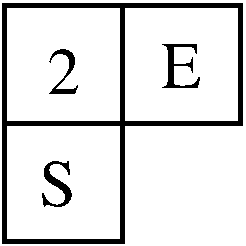
\includegraphics[height=0.4in,width=0.4in, keepaspectratio]{L2.pdf}
   \item['3'] se le due celle periferiche sono etichettate 'S' e 'W'. Il tromino \`e 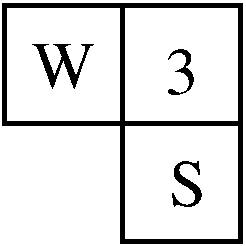
\includegraphics[height=0.4in,width=0.4in, keepaspectratio]{L3.pdf}
   \item['4'] se le due celle periferiche sono etichettate 'W' e 'N'. Il tromino \`e 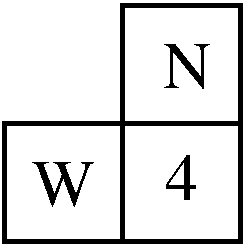
\includegraphics[height=0.4in,width=0.4in, keepaspectratio]{L4.pdf}  
\end{itemize}


% Assunzioni
\section*{Assunzioni}

\begin{itemize}
   \item righe e colonne sono numerate da $0$ a $2^k -1$.  
   \item $k\leq 10$.
\end{itemize}

% Subtasks
\section*{Subtask}
\begin{itemize}
\item \textbf{Subtask 1 [0 punti]:} caso di esempio.
\item \textbf{Subtask 2 [10 punti]:} $k = 2$.
\item \textbf{Subtask 3 [40 punti]:} il buco \`e collocato in angolo della scacchiera $2^k\times 2^k$.
\item \textbf{Subtask 4 [10 punti]:} $k = 3$ (scacchiera $8\times 8$).
\item \textbf{Subtask 5 [40 punti]:} $k \leq 10$.
\end{itemize}

% Esempi
\section*{Esempio di input/output}
\esempio{3 1 1}{\scriptsize
2EW32EW3

S0NSSW3S

NW4NW3SN

1EW4NSW4

2ENW4NW3

SN1EW4NS

N1ENNW4N

1EW41EW4
}

\end{document}
